\documentclass[a4paper,11pt]{article}

\usepackage[utf8]{inputenc}	
\usepackage[T1]{fontenc}
\usepackage{lmodern}
\usepackage{times}
\usepackage[margin=2cm]{geometry}
\usepackage{amsmath}
\usepackage{mathtools}
\usepackage{graphicx}
\usepackage{multirow}
\usepackage{blindtext}
\usepackage{hyperref}

\usepackage{pgfplotstable} 
\usepackage{booktabs}

\graphicspath{ {./images/} }

\usepackage[czech]{babel}
\usepackage{graphicx}
\usepackage{amsmath}
\usepackage{xspace}
\usepackage{url}
\usepackage{indentfirst}
\usepackage{subcaption}
\usepackage{caption}
\usepackage{tabularx}
\usepackage{rotating}
\usepackage{tikz}
\usepackage[labelformat=parens,labelsep=quad,skip=3pt]{caption}

\usepackage{color}  
\usepackage{listings}

\definecolor{codegreen}{rgb}{0,0.6,0}
\definecolor{codegray}{rgb}{0.5,0.5,0.5}
\definecolor{codepurple}{rgb}{0.58,0,0.82}
\definecolor{backcolour}{rgb}{0.95,0.95,0.92}

\lstdefinestyle{mystyle}{
    backgroundcolor=\color{backcolour},   
    commentstyle=\color{codegreen},
    keywordstyle=\color{magenta},
    numberstyle=\tiny\color{codegray},
    stringstyle=\color{codepurple},
    basicstyle=\ttfamily\footnotesize\centering,        
    breaklines=true,                 
    captionpos=b,                                  
    numbers=left,                    
    numbersep=5pt,                  
    showspaces=false,              
    showstringspaces=false,
    showtabs=false,                  
    tabsize=2
}

\lstset{style=mystyle}


\widowpenalty 10000 \clubpenalty 10000 \displaywidowpenalty 10000
\setcounter{topnumber}{3}	  
\setcounter{bottomnumber}{3}	 
\setcounter{totalnumber}{6}	  
\renewcommand\topfraction{0.9}	 
\renewcommand\bottomfraction{0.9} 
\renewcommand\textfraction{0.1}	  
\intextsep=8mm \textfloatsep=8mm 

\renewcommand{\thesection}{\arabic{section}.}
\renewcommand{\thesubsection}{\thesection\arabic{subsection}.}
\makeatletter \def\@seccntformat#1{\csname the#1\endcsname\hspace{1ex}} \makeatother


\begin{document}

\hline
\begin{center}
\bigskip
\huge Popisná statistika I
\vspace{0.5cm}
\par \large F7581 Praktická astrofyzika - základy
\par \large Artem Gorodilov
\vspace{0.5cm}
\par \large 7. ~října 2024
\bigskip
\end{center}
\hline
\bigskip


\vskip10pt
    \begin{minipage}[t]{0.5\textwidth} 
        Pro statistickou analýzu jsme měli k dispozici data uvedená v tabulce (1).
        \par a) Hodnota extinkčního koeficientu byla měřena 20krát. Údaje mají spojitý charakter. 
        \par b) Váhy byly vypočteny pomocí koeficientu K = 0.00169.
        \par c) Vypočítali jsme aritmetický průměr $y_m$, vážený aritmetický průměr $y_{mw}$, nejistotu aritmetického průměru $md$, nejistotu váženého aritmetického průměru $wmd$, geometrický průměr $y_{mG}$, harmonický průměr $y_{mH}$, kvadratický průměr $y_{mQ}$, medián $med(y)$ a vážený medián $wmed(y)$:
        \begin{center}
            $y_m$ = 0.4805, $y_{mw}$ = 0.5007,
            \vspace{5pt}
            \par $md$ = 0.15565, $wmd$ = 0.15062,
            \vspace{5pt}
            \par $y_{mG}$ = 0.43499, $y_{mH}$ = 0.38164, $y_{mQ}$ = 0.52207,
            \vspace{5pt}
            \par $med(y)$ = 0.425, $wmed(y)$ = 0.41.
        \end{center}
        \par d) Minimální a maximální hodnoty extinkce a celkové roypětí:
        \begin{center}
            $y_{min}$ = 0.11, $y_{max}$ = 0.97, $y_{range}$ = 0.86.
        \end{center}
        \par e) Rozptyl $s$ a $s_w$, odhad disperze $\sigma$, střední velikost odchylky s centrem v aritmetickém průměru $md$ a $wmd$, medián $mad$ a $wmad$:
        \begin{center}
            $s$ = $\sigma$ = 0.2095, $s_w$ = 0.2012,
            \vspace{5pt}
            \par $md$ = 0.15565, $wmd$ = 0.15062,
            \vspace{5pt}
            \par $mad$ = 0.095, $wmad$ = 0.13.
        \end{center}
        \par f) Vykreslili jsme graf kumulativních distribuční funkce, které je vidět na obrázku (\ref{fig:com_dist}). Hodnoty kvartilů $Q_1$ a $Q_3$ a mezikvartilního rozpěti $Q_2$:
        \begin{center}
            $Q_1$ = 0.39, $Q_3$ = 0.5475, $Q_2$ = 0.425.
        \end{center}

        \par g) Hodnoty středu rozdělení $\mu$ jsme zjistili pomocí aritmetického průměru $\mu_a$ a mediánu $\mu_m$:
        \begin{center}
            $\mu_a$ = 0.4805, $\mu_m$ = 0.425.
        \end{center}
    \end{minipage}
    \hspace{10pt}
    \begin{minipage}[t]{0.5\textwidth} 
        \vspace{10pt}   
        \par \centering
        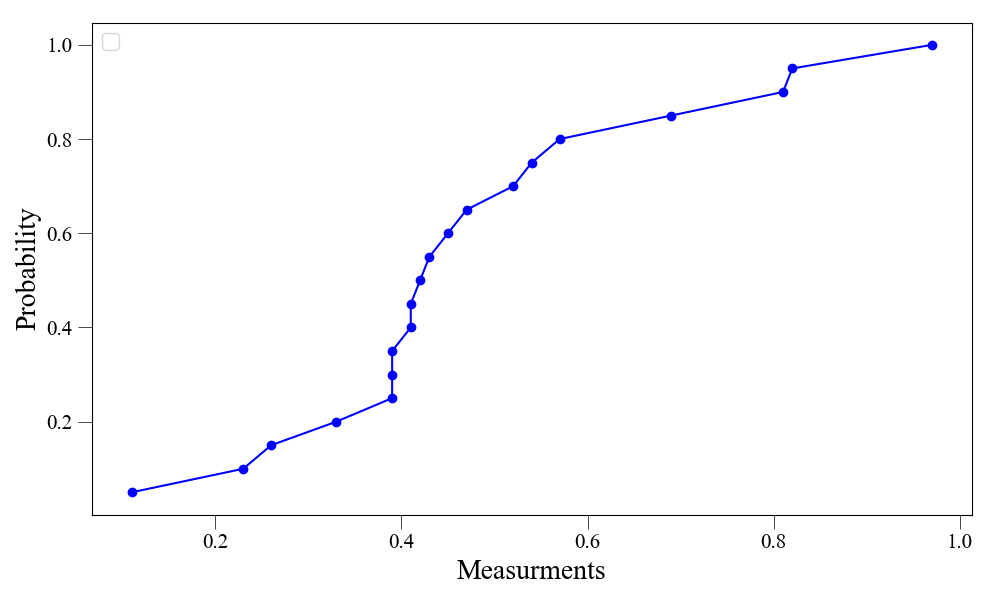
\includegraphics[scale=0.33]{com_dist}
        \captionsetup{justification=centering, font=footnotesize}
        \captionof{figure}{Kumulativní distribuční funkce}
        \label{fig:com_dist}
        \vspace{10pt}
        \raggedright 
        
        \par Disperzi rozdělení $\sigma$ jsme zjistili pomocí střední odchylky $\sigma_s$ a vážené střední odchylky $\sigma_w$:
        \begin{center}
            $\sigma_s$ = 0.2149, $\sigma_w$ = 0.2064.
        \end{center}
        \par h) Histogram byl vykreslen s počtem tříd $n$ = 5 a šířkou třídy $h$ = 0.2. Výsledek je vidět na obrázku (\ref{fig:histogram}).

        \vspace{10pt}   
        \par \centering
        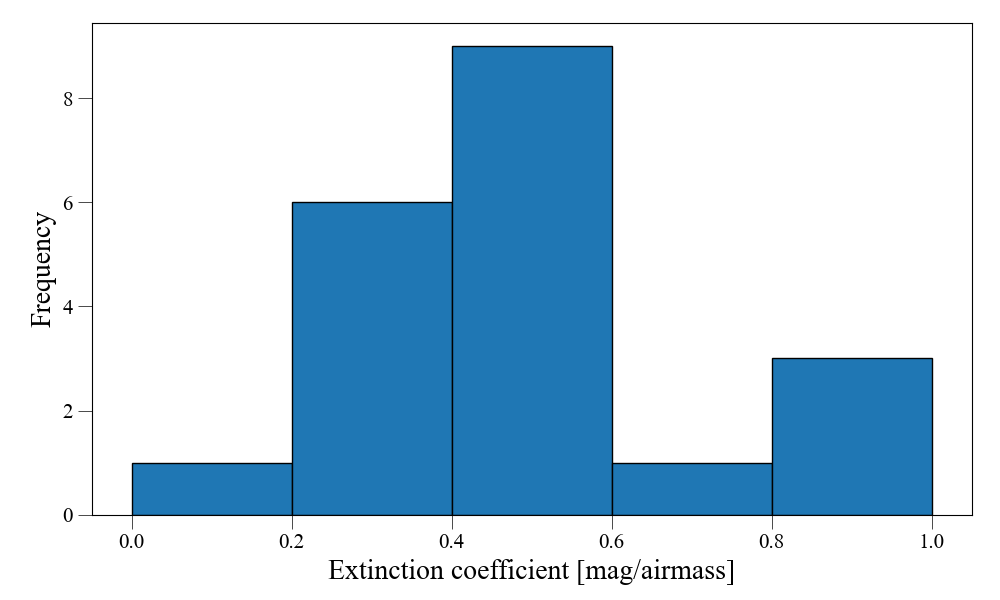
\includegraphics[scale=0.33]{histogram}
        \captionsetup{justification=centering, font=footnotesize}
        \captionof{figure}{Histogram s počtem tříd $n$ = 5 a šířkou třídy $h$ = 0.2}
        \label{fig:histogram}
        \vspace{10pt}
        \raggedright 

        \par i) Modus $Mo$ je roven:
        \begin{center}
            $Mo$ = 0.39, $count(Mo)$ = 3.
        \end{center}

        \par j) Z rozdělení je patrné, že většina hodnot extinkce je vyšší než 0.262 [mag/airmass]. To znamená, že kromě Rayleighová rozptylu se na extinkci podílejí další jevy.
    \end{minipage}

    \begin{center}
            \section{Tabulka naměřených hodnot pro spektrální čáry železa}
                \pgfplotstabletypeset[
                col sep=comma, 
                string type, 
                every head row/.style={before row=\toprule,after row=\midrule},
                every last row/.style={after row=\bottomrule},
                columns/val/.style={column name=A [mag/airmass]},
                columns/err/.style={column name=A$_{err}$ [mag/airmass]},
                columns/weight/.style={column name=Weight},
                ]{data/data_proc.csv}
    \end{center}
\end{document}